%========================================
% Beamer "Singapore" Theme Template
%========================================
\documentclass[aspectratio=169]{beamer}

% THEME
\usetheme{Singapore}

% COLORS & FONTS
\definecolor{brand}{RGB}{45,110,191}
\definecolor{accent}{RGB}{5,155,192}
\definecolor{hrgray}{RGB}{100,100,100}
\setbeamercolor{structure}{fg=brand}
\setbeamercolor{title}{fg=hrgray}
\setbeamercolor{subtitle}{fg=brand}
\setbeamercolor{author}{fg=hrgray}
\setbeamercolor{date}{fg=hrgray}
\setbeamercolor{frametitle}{fg=hrgray}
\setbeamercolor{block title}{fg=white,bg=brand}
\setbeamercolor{block body}{bg=black!2}
\usepackage{lmodern}
\usefonttheme{professionalfonts}

\usepackage{comment}
\usepackage{etoolbox}
\usepackage[T1]{fontenc}
\usepackage[utf8]{inputenc}
\usepackage{microtype}
\usepackage{graphicx}
\usepackage{tikz}
\usepackage{xcolor}

\setbeamertemplate{navigation symbols}{}

\setbeamertemplate{footline}{
  \leavevmode
  \hbox{
    \begin{beamercolorbox}[wd=.5\paperwidth,ht=3ex,dp=1ex,left]{author in head/foot}
      \hspace{0.8ex}{
\includegraphics[height=0.5cm]{img/logo.png}}
    \end{beamercolorbox}%
    \begin{beamercolorbox}[wd=.5\paperwidth,ht=3ex,dp=1ex,right]{date in head/foot}
      \insertframenumber{} / \inserttotalframenumber\hspace{2ex}
    \end{beamercolorbox}%
  }
  \vskip0pt
}

% METADATA
\title[Short Title]{\bfseries{Human-AI Teaming Seminar 1}}
\subtitle{Basic Chatbot Usage}
\author[Patrick Hall]{\textbf{Patrick Hall}}
\institute{George Washington School of Business}
\date{\today}

% handle URLs/links
\PassOptionsToPackage{hyphens}{url}\usepackage{hyperref}
\urlstyle{same}
\hypersetup{
    colorlinks=true,
    urlcolor=[rgb]{0.0196, 0.6078, 0.7529},
    linkcolor=[rgb]{0.17647, 0.388, 0.749},
    citecolor=[rgb]{0.0196, 0.6078, 0.7529}
}

% Chicago citations and bibliography
\setbeamertemplate{bibliography item}[text]
\usepackage[authordate]{biblatex-chicago}
\setbeamertemplate{frametitle continuation}{}
\addbibresource{references.bib}
\setlength{\bibitemsep}{0.5\baselineskip}
\AtBeginBibliography{\scriptsize}
\renewcommand\UrlFont{\sffamily}

\begin{document}

%-------------------------
\begin{frame}

  \titlepage
  \begin{tikzpicture}[remember picture,overlay]
    \node[opacity=0.1] at (current page.center)
      {
\includegraphics[width=0.55\paperwidth]{img/logo.png}};
  \end{tikzpicture}
  \centering\footnotesize{\color{hrgray}{\textcopyright~2025-26 Patrick Hall (jphall@gwu.edu). Some rights reserved.\\Text and copy are licensed under a Creative Commons Attribution-NonCommercial-ShareAlike 4.0 International License (CC BY-NC-SA 4.0).}}

\end{frame}

%-------------------------
\begin{frame}{Agenda}\small
  \tableofcontents
  \vspace{10pt}
  \textbf{Optional Prerequisites:} access to Copilot or Gemini \href{https://tinyurl.com/3zvh5b47}{chatbots} through GW, free \href{https://www.overleaf.com/}{Overleaf} account or your favorite LaTeX Editor, and Google Colab and \href{https://drive.google.com}{Drive} through GW.   
  
\end{frame}

\section{GW AI Tools and Policies}

\begin{frame}{GW AI Tools and Policies}

    \Large
    GW guidance on approved tools, data, and classroom use:\\ 
    \begin{itemize}
        \item \href{https://tinyurl.com/3zvh5b47}{AI Tools and Services (Approved Tools List)}.\\
        \item \href{https://it.gwu.edu/data-classification-guide}{Data Classification Guidelines}.\\
        \item \href{https://library.gwu.edu/generative-ai}{Generative Artificial Intelligence (GW Libraries)}.\\
    \end{itemize}
    \vspace{10pt}
    GW also provides resources for \href{https://provost.gwu.edu/sites/g/files/zaxdzs5926/files/2023-04/generative-artificial-intelligence-guidelines-april-2023.pdf}{syllabus statements}, \href{https://sites.google.com/view/aiassignments}{assignments}, and other common activities.
    
\end{frame}

\section{Decision Making and Overreliance}

%------------------------------------------------
\begin{frame}[t]{Chatbots — Avoid Overreliance for Decision Making\\
\small{\parencite{TowardsaStandardforI537, ArtificialIntelligen058}}}
\textbf{Principle:} Fundamentally, chatbots guess the next word \parencite{hicks2024chatgpt}. Don’t let chatbots replace your reasoning and judgment. But you can use them to augment your own thinking.

\vspace{1em}

\textbf{Use Chatbots for:}
\begin{itemize}
    \item Advice on options — you select the best option using real-world knowledge.
    \item Feedback and improvement on your own ideas or decisions.
    \item Assistance structuring decision-making processes.
    \item In general, combine your own reasoning with statistical, machine learning, or optimization approaches (like predictive models or chatbots) as decision-support mechanisms. 
\end{itemize}

\vspace{1em}

\textbf{Decision-making mini-exercise.} 

\end{frame}

%------------------------------------------------
\begin{frame}[t]{Chatbots — Decision-Making Mini-exercise}

\footnotesize
Start with a polite salutation and orient the chatbot to the subject at hand: ``\texttt{Hi, are you familiar with the subject X?}'' \parencite{please_be_polite_chatgpt_2024}\\
\vspace{1em}
If possible, provide background information in bullets or short clear statements: ``\texttt{Here is my current thinking on X...}''\\ 
\vspace{1em}
Consider asking for options: ``\texttt{Given my current thinking, can you provide me some reasonable options for proceeding with X?}''\\ 
\vspace{1em}
Consider asking for feedback: ``\texttt{Given my current thinking, can you provide feedback on what I may be missing or getting wrong about X?}''\\
\vspace{1em}
Consider asking about how decisions are made about X: ``\texttt{Are there any well-known or accepted processes for deciding about X?}''\\ 
\vspace{1em}
\textbf{Reminder: No sensitive or personal information!} 

\end{frame}

\section{Search and Factual Requests}

%------------------------------------------------
\begin{frame}[t]{Chatbots — Search and Factual Requests}
\begin{columns}[T]
    \column{0.58\textwidth}
    \textbf{Don’t let chatbots answer factual requests for you} \parencite{graydon2025examining}.

    \vspace{1em}

    \textbf{Instead:}
    \begin{itemize}
        \item Use credible search engines (Wayback Machine, Google Scholar).
        \item Consult libraries, books, indices, and databases.
        \item Consult human experts (e.g., professors, reference librarians).
    \end{itemize}

    \vspace{1em}
    \textit{Chatbots can assist — but should not be the source of record.}

    \column{0.42\textwidth}
    \centering
    
\includegraphics[width=0.8\linewidth]{img/bad_search.jpg}\\
    \scriptsize A notorious Google AI search failure.
\end{columns}
\end{frame}

\section{Writing Workflows}

%------------------------------------------------
\begin{frame}[t]{Chatbots — Writing Workflows}
\textbf{Don’t let chatbots write for you} \parencite{alkaissi2023artificial}.

\vspace{1em}

\textbf{Recommended workflow:}
\begin{itemize}
    \item You create the outline.
    \begin{itemize}
        \item You add citations, figures, tables, and validation.
    \end{itemize}
    \item Chatbots draft the outline into coherent text.
    \item You proofread and edit.\\
\end{itemize}
\vspace{5pt}
OR\\ 
\vspace{10pt}
Ask chatbots for feedback, critique, and editing help. Use tools like Grammarly for more thorough copy-editing.\\ 
\vspace{1em}
\textbf{Writing mini-exercise.} 
\end{frame}

%------------------------------------------------
\begin{frame}[t]{Chatbots — Writing Mini-exercise}

\footnotesize
Start with a polite salutation and orient the chatbot to the writing exercise at hand: ``\texttt{Hi, I need help converting outline bullets into a paragraph of text for a blog post about X.}''\\
\vspace{1em}
Gather references, create tables and figures, and compose materials into an outline. Ask the chatbot to draft your bullets into paragraphs, referencing the provided tables, figures, and citations, and if necessary, to avoid creating any new tables, figures, and citations. \\
\vspace{1em}
If using a technical format, e.g., LaTeX or asciidoc, have the chatbot generate this format directly.\\
\vspace{1em}
OR\\
\vspace{1em}
Ask a chatbot to edit or provide feedback on something you have drafted. Ask for help with flow, concision, clarity, transitions, appropriateness for audience, omissions, etc.\\
\vspace{1em} 
\textbf{Reminder: You should proof and edit any chatbot-generated text, and be especially careful with citations.} 

\end{frame}

\section{Coding Workflows}

%------------------------------------------------
\begin{frame}[t]{Chatbots — Coding Workflows}
\textbf{Don’t blindly trust AI to code for you} \parencite{graydon2025examining}.
\vspace{1em}

\textbf{More thoughtful approaches:}
\begin{itemize}
    \item AI writes code; you write tests and documentation. To retain traceability: 
    \begin{itemize}
        \item Have AI write code for you incrementally---function-by-function, module-by-module.
        \item Keep each block of functionality runnable or testable on its own.
    \end{itemize}
    \item You write code; AI writes tests and documentation.
    \item AI ``pair programming:'' Have AI implement the same logic two different ways and verify matching outputs.\\
\end{itemize} 
\vspace{1em}
\textbf{``Hello World'' mini-exercise.} 
\end{frame}

\section{Common Pitfalls}

%------------------------------------------------
\begin{frame}[t]{Chatbots — When to Use Other Tools}
\textbf{Understand when to use other types of AI.}

\begin{columns}[T]
    \column{0.55\textwidth}
    \vspace{1em}
    \begin{itemize}
        \item Optimization, statistics, and ML for data analysis and decision making.
        \item Real-time sensor systems for live information (traffic, weather, etc.).
        \item Credible search systems for factual retrieval.
    \end{itemize}

    \vspace{1em}
    People can overrely on reasoning when basic data analysis could lead to better decisions, e.g., the representativeness heuristic.

    \column{0.45\textwidth}
    \centering
    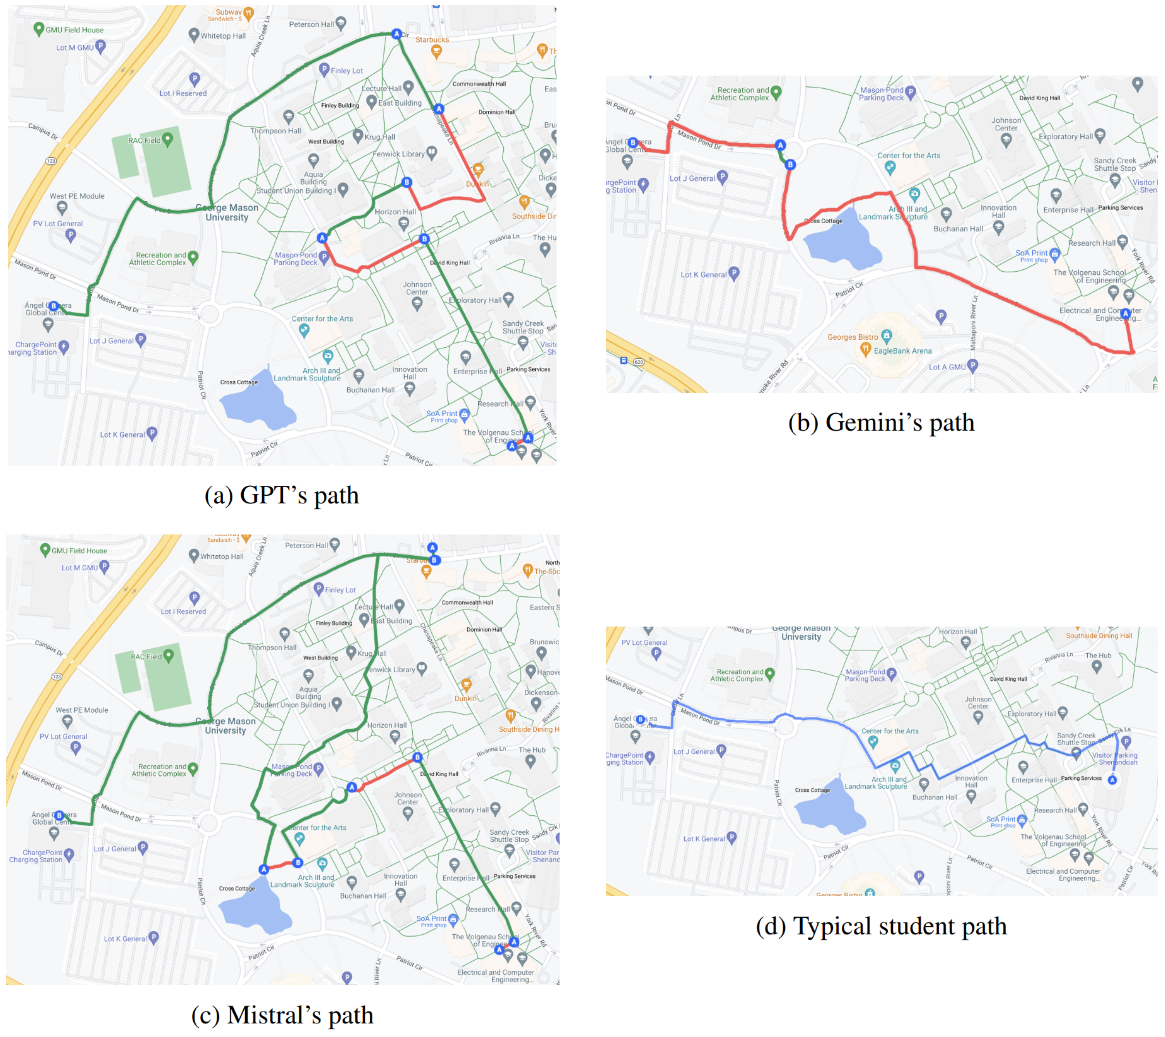
\includegraphics[width=0.8\linewidth]{img/bad_map.png}\\
    \scriptsize Illogical mapping decisions from language models on GMU campus \parencite{chen2024can}.
\end{columns}
\end{frame}

%------------------------------------------------
\begin{frame}[t]{Chatbots — Common AI Fails\\
\small{\parencite{TowardsaStandardforI537, ArtificialIntelligen058}}}
\begin{columns}[T]
    \column{0.5\textwidth}
    \textbf{How AI Fails You}
    \vspace{0.8em}
    \begin{itemize}
        \item Hallucinating or fabricating information.
        \item Generating fake citations.
        \item Combining true information incorrectly.
        \item Poor knowledge in niche domains.
        \item Failing at complex reasoning tasks.
        \item Misusing or exposing sensitive information.
    \end{itemize}

    \column{0.5\textwidth}
    \textbf{How You Fail with AI}
    \vspace{0.8em}
    \begin{itemize}
        \item Allowing outputs to confirm pre-existing biases.
        \item Anthropomorphizing AI (AI does not ``think,'' ``understand,'' ``feel''), including emotional entanglement.
        \item Anchoring to AI outputs as first-seen information.
        \item Accepting sycophantic responses.
        \item Inputting sensitive information.
    \end{itemize}
\end{columns}
\end{frame}

%------------------------------------------------
\begin{frame}{Chatbots — How AI Differs from Human Thinking \parencite{bennett2023brief}}
\begin{itemize}
    \item Lacks a model of the physical world.
    \begin{itemize}
        \item But this is being worked on (e.g, \href{https://www.nvidia.com/en-us/ai/cosmos/}{NVIDIA Cosmos}).
    \end{itemize}
    \item Lacks a model of its own information processing.
    \begin{itemize}
        \item But does approximate via ``Chain-of-Thought'' (CoT) workflows \parencite{wei2022chain}.
    \end{itemize}
    \item Lacks emotional motivation.
    \item Uses different sensory inputs and outputs (digital data vs. human senses).
    \item Can use massive memory.
    \item Can perform repetitive cognitive tasks without fatigue.
\end{itemize}
\end{frame}

% references
\begin{frame}[t, allowframebreaks]{References}
  \printbibliography[heading=none]
\end{frame}


\end{document}
